\section{Experiments}\label{sec:experiments}

\subsection{Data}\label{sec:data}

{\color{red}{\color{black}
We evaluate at one-minute resolution, in contrast to the daily
frequency used in most existing evaluations of synthetic financial
time series.}
{\color{black}The real data consist of one-minute close prices for U.S.-listed equities
obtained from Alpaca's SIP feed, restricted to regular trading hours on
the NYSE calendar.}
{\color{black}The sample covers September~3, 2019 through March~20, 2020, comprising
139~trading sessions.}
{\color{black}This period includes both relatively calm market conditions and the onset
of the COVID-19 disruption, allowing the evaluation to examine statistical
fidelity across different volatility conditions.}
{\color{black}The real and AIL datasets have 948~tickers in common.}
{\color{black}From this overlap, we retain the 600~tickers for which both series attain
at least 70\% non-missing coverage on the common one-minute market clock.}
{\color{black}The resulting universe is used throughout the empirical comparison.}
{\color{black}Missing observations are retained rather than imputed.}
For M3, the common 360-return support excludes the two early-close
sessions, November~29 and December~24, 2019, which cannot supply the
required interval.
This leaves 137 full-length sessions eligible for M3;
the same support rule is applied to the real and all synthetic panels.
This exclusion is specific to M3 and does not remove those dates from the
other metrics.
}

All panels are processed under the same conditional preprocessing rule.
Returns are log-price differences between adjacent observed closes, with the first return of each session masked to exclude the overnight gap.
Since close-price observations begin at 09:31, the return timestamped 09:31 is structurally unavailable and is masked, leaving 389 valid close-to-close returns from 09:32 to 16:00.

Intraday volatility seasonality is detected separately in each panel from the coefficient of variation of its minute-of-session variance profile.
When seasonality is detected, a four-harmonic Flexible Fourier Form regression \citep{andersen1997intraday} is fitted independently per series by linear least squares.
The fitted volatility multiplier is normalized to unit mean squared scale before deseasonalization, approximately preserving the series' overall variance.
Non-seasonal panels, including GBM and MSV, are left unchanged.

\subsection{Generators}\label{sec:generators}

To benchmark our framework we use multiple generators, using both state
of the art and baseline models.

\paragraph{Brownian Motion (GBM):}
Log-return increments are drawn independently from a Normal
distribution, with mean and variance estimated per ticker from the
real data.
The resulting series has no volatility clustering, no heavy tails
beyond the Gaussian, and no regime-dependent tail structure, by
construction.
A generator that fails to separate from GBM on a given metric provides
no signal beyond that of independent Gaussian noise under that metric.

\paragraph{Multi-Scale Stochastic Volatility model (MSV):}
This generator follows a two-timescale construction in the spirit of
\citet{fouque2000derivatives}.
Its log-volatility combines a slow factor, persistent across trading sessions, with a fast factor that decays within a session.
This structure is designed to reproduce the slow decay of absolute-return autocorrelation targeted by M2.
\edited{The slow factor is fractional Gaussian noise across session dates,
held constant within each session, with Hurst exponent $H=0.90$.
The fast factor is a stationary intraday AR(1) process with
$\phi=\exp(-1/\tau_{\mathrm{fast}})$ and
$\tau_{\mathrm{fast}}=20$ minutes.
Their log-volatility amplitudes are
$\nu_{\mathrm{slow}}=0.9$ and $\nu_{\mathrm{fast}}=0.3$, respectively.
These settings specify the persistence and relative strength of the two
volatility components; the ticker-specific scaling separately matches
the real return standard deviation.}
The factor parameters were selected by matching
the simulated and real absolute-return autocorrelation curves, while the
unconditional return scale was calibrated per ticker.
MSV therefore serves
as a model-based positive control for M2: it tests whether the metric assigns
a comparatively high score to a generator explicitly designed to reproduce
the dependence structure it measures.
Unlike a resampled-real control, it
still generates new observations from a stochastic-volatility model rather
than reusing historical returns.
Since MSV has no deterministic
minute-of-session volatility profile, it is left unchanged by the conditional
deseasonalization step.


\paragraph{AIL:} To be filled.

\paragraph{Schr\"odinger--Bass Bridge for Time Series (SBBTS):}
\edited{{\color{black}This generator implements Algorithm 1 of \citet{alouadi2026sbbts}.}
{\color{black}A drift network, conditioned on the past trajectory through a one-layer
causal transformer encoder, is trained on standardized cumulative
log-return paths, one per ticker and full-length session of the real
panel.}
{\color{black}Missing minutes are dropped rather than imputed, so the time grid is
irregular, and we therefore replace the index-based positional encoding
of the original paper with an elapsed-time embedding.}
{\color{black}In each outer iteration the endpoint transform is computed from a frozen,
detached copy of the previous iterate, which differs from the reference
implementation of the authors.}
{\color{black}The most recent 20\% of session dates are held out for early stopping.}
These dates, February~12 through March~20, 2020, are held out from
parameter fitting but remain inside the evaluation window.
Thus, the
early-stopping split is not an independent evaluation holdout: model
selection has access to this period, including the onset of the COVID-19
crash.
{\color{black}We train five outer iterations and use the final one, as returned by
Algorithm 1.}
The historical training record has its smallest logged validation minimum
at the fourth iteration (5.6388, epoch 8), compared with 5.7248 at epoch 12
of the fifth iteration.
These losses use different frozen-transform regression targets and
validation noise across iterations, so their raw minima are not a common
criterion for selecting the outer iteration.
Early stopping selects an epoch within each iteration; the evaluated
panel is retained under the fixed final-iteration protocol.
{\color{black}Each generated path is rescaled by the training scale of its ticker,
anchored at the first observed real price of the session, and given the
missingness mask of the real panel.}
{\color{black}Training and generation are run once, so the outer-bootstrap intervals
do not include generator uncertainty.}}


% RUN4-VERIFIED: O=200, M=20; source tables archived in deliverables/reproducibility/run4/.
\subsection{Evaluation Protocol}\label{sec:experiments_protocol}

\edited{We frame the comparison as an in-sample empirical fidelity
assessment over the full September~3, 2019--March~20, 2020 window.
It measures how well the fixed synthetic panels reproduce the statistical
properties of this historical corpus, including the dates used for SBBTS
early stopping.
We do not interpret the scores as evidence of
out-of-sample generalisation to unseen trading dates.
The M3 support
restriction described above remains metric-specific.}

We evaluate each generator using $R=100$ matched inner draws with a subsample size of $n=200$ ticker columns per panel. Within every draw, the first real subsample is shared between the real–real and synthetic–real comparisons, while the second real subsample and each synthetic subsample are drawn independently.

Point estimates are computed on the original preprocessed panels. \edited{We quantify uncertainty with respect to ticker-corpus composition using $O=200$ outer bootstrap replicates.} In each replicate, the complete real panel and each complete synthetic panel are resampled independently by ticker with replacement, retaining their original numbers of columns. The full $R$-draw matched estimator is then recomputed on the resulting outer-resampled panels. We report the 2.5th–97.5th percentile range of the outer scores as the 95\% confidence interval.

\edited{We additionally evaluate numerical stability over $M=20$ independent inner-resampling seeds while holding the observed corpora fixed.
The root seed is 42; repeat zero reuses its point estimate, and 19 further seeds are drawn from a separate deterministic random stream.
We report the resulting standard deviation and range separately as Monte Carlo stability diagnostics rather than confidence intervals.}

All random streams are derived deterministically from the root seed and their statistical role. Random indices are generated independently of task-completion order, so parallel execution, worker count, and chunking do not alter the samples assigned to an evaluation or replicate.

Table~\ref{tab:config} collects the metric and protocol parameters
deferred from Section~\ref{sec:method}.

\begin{table}[htbp]
\centering
\caption{Metric and protocol parameters \edited{used in the completed evaluation.}}
\label{tab:config}
\small
\begin{tabular}{@{}llr@{}}
\toprule
Component & Parameter & Value \\
\midrule
Preprocessing & Intraday-seasonality CV threshold & 0.30 \\
Scoring protocol & Evaluation draws, $R$ & 100 \\
                 & Subsample size, $n$ & 200 \\
                 & Outer corpus bootstrap replicates, $O$ & 200 \\
                 & Independent inner-seed repeats, $M$ & 20 \\
\addlinespace
M1 & Quantile grid resolution, $J$ & 5\,001 \\
   & Tail-emphasis sharpness, $\alpha$ & 0.3 \\
   & Tail-emphasis magnitude, $\lambda$ & 1.0 \\
\addlinespace
M2 & Lag window, $[k_{\min}, k_{\max}]$ & $[60, 388]$ \\
\addlinespace
M3 & Aggregation scales, $\mathcal{H}$ & $\{1, 5, 15, 30\}$ \\
   & Minimum pooled observations & 100 \\
\addlinespace
M4 & Rolling-volatility window & 60 \\
   & Minimum valid fraction & 0.5 \\
   & Volatility regimes, $|\mathcal{Q}|$ & 5 \\
   & Tail quantile & 0.05 \\
   & Minimum exceedances per regime & 500 \\
   & Regime weights & $1{:}1{:}1{:}2{:}3$ \\
\bottomrule
\end{tabular}
\par\vspace{2pt}
\footnotesize
Lags, windows, and scales are in minutes. Regime weights run from the
calmest to the most turbulent quintile and are normalized to sum to one.
\end{table}


% RUN4-VERIFIED-RESULTS: Generated table values checked against the archived CSVs.
\subsection{Results}\label{sec:results}

{\color{red}
Table~\ref{tab:scores} reports the four stylized-fact similarity scores
and the aggregate deviation score $G_{\mathrm{dev}}$.
The intervals describe variation under ticker-corpus resampling,
conditional on the fitted preprocessing transformations and the available
generator outputs.
A similarity score of $0.5$ corresponds to equal estimated
synthetic--real and real--real resampling gaps; a lower score indicates
a larger synthetic--real discrepancy.
All 200 outer replicates retained 100 valid matched draws for every
metric--generator combination.
}

\begin{table}[htbp]
\centering
\color{red}
\caption{Similarity scores $s_k$ and aggregate deviation score $G_{\mathrm{dev}}$ for each generator. Point estimates use $R=100$ matched draws with $n=200$ tickers and root seed 42. Brackets contain 95\% outer ticker-corpus percentile-bootstrap intervals from $O=200$ replicates; these differ from the seed-stability diagnostics in Appendix~\ref{app:reproducibility}.}
\label{tab:scores}
\small
\setlength{\tabcolsep}{3pt}
\begin{tabular*}{\textwidth}{@{\extracolsep{\fill}}lcccc@{}}
\toprule
 & AIL & GBM & MSV & SBBTS \\
\midrule
M1 & 0.3436 & 0.0184 & 0.0790 & 0.0245 \\
\footnotesize Marginal distribution & \footnotesize[0.2892, 0.4292] & \footnotesize[0.0178, 0.0225] & \footnotesize[0.0753, 0.0971] & \footnotesize[0.0237, 0.0300] \\
\addlinespace
M2 & 0.2136 & 0.0186 & 0.2925 & 0.0203 \\
\footnotesize Volatility clustering & \footnotesize[0.1726, 0.3482] & \footnotesize[0.0183, 0.0237] & \footnotesize[0.2400, 0.3664] & \footnotesize[0.0200, 0.0259] \\
\addlinespace
M3 & 0.3622 & 0.1025 & 0.1294 & 0.2872 \\
\footnotesize Gaussianity & \footnotesize[0.2445, 0.4912] & \footnotesize[0.0702, 0.1433] & \footnotesize[0.0885, 0.1865] & \footnotesize[0.1904, 0.4074] \\
\addlinespace
M4 & 0.4818 & 0.0384 & 0.0929 & 0.1245 \\
\footnotesize Conditional tails & \footnotesize[0.3922, 0.5053] & \footnotesize[0.0349, 0.0438] & \footnotesize[0.0833, 0.1042] & \footnotesize[0.1114, 0.1396] \\
\addlinespace
\midrule
$G_{\mathrm{dev}}$ & 1.911 & 28.031 & 6.561 & 13.532 \\
\footnotesize Aggregate deviation & \footnotesize[1.522, 2.325] & \footnotesize[23.750, 30.219] & \footnotesize[5.541, 7.277] & \footnotesize[11.220, 14.722] \\
\bottomrule
\end{tabular*}
\end{table}

{\color{red}
The Gaussian control receives low scores across all four properties,
with intervals well below $0.5$.
Its M1 and M2 point scores are $0.0184$ and $0.0186$, respectively,
while its M3 and M4 scores are $0.1025$ and $0.0384$.
These results are consistent with the absence of heavy-tailed
innovations, persistent absolute-return dependence, and
regime-dependent tail structure in GBM.
The negative control therefore checks that the framework responds to
known deficiencies rather than assigning high similarity to
independent Gaussian returns.
MSV improves on GBM across all four metrics.
Its clearest relative strength is volatility clustering: the M2 score
is $0.2925$, compared with $0.2136$ for AIL, although the marginal
intervals overlap ($[0.2400,0.3664]$ and $[0.1726,0.3482]$).
This ordering is descriptive; the reported intervals do not provide a
paired test of the difference between generators.
Since MSV was calibrated to the real absolute-return autocorrelation,
its M2 performance provides a positive-control check of responsiveness
to the dependence structure targeted by the metric.

Figure~\ref{fig:m2-acf} provides a descriptive view of the absolute-return
dependence underlying M2. The full-panel MSV curve tracks the real curve
closely over the comparison window, while AIL generally lies below it.
SBBTS exhibits substantially weaker persistence and GBM remains near zero.
These profiles identify the direction of the discrepancies; the scores
and intervals in Table~\ref{tab:scores} additionally calibrate the matched
synthetic--real gaps against real--real variation.
\begin{figure}[tbp]
\centering
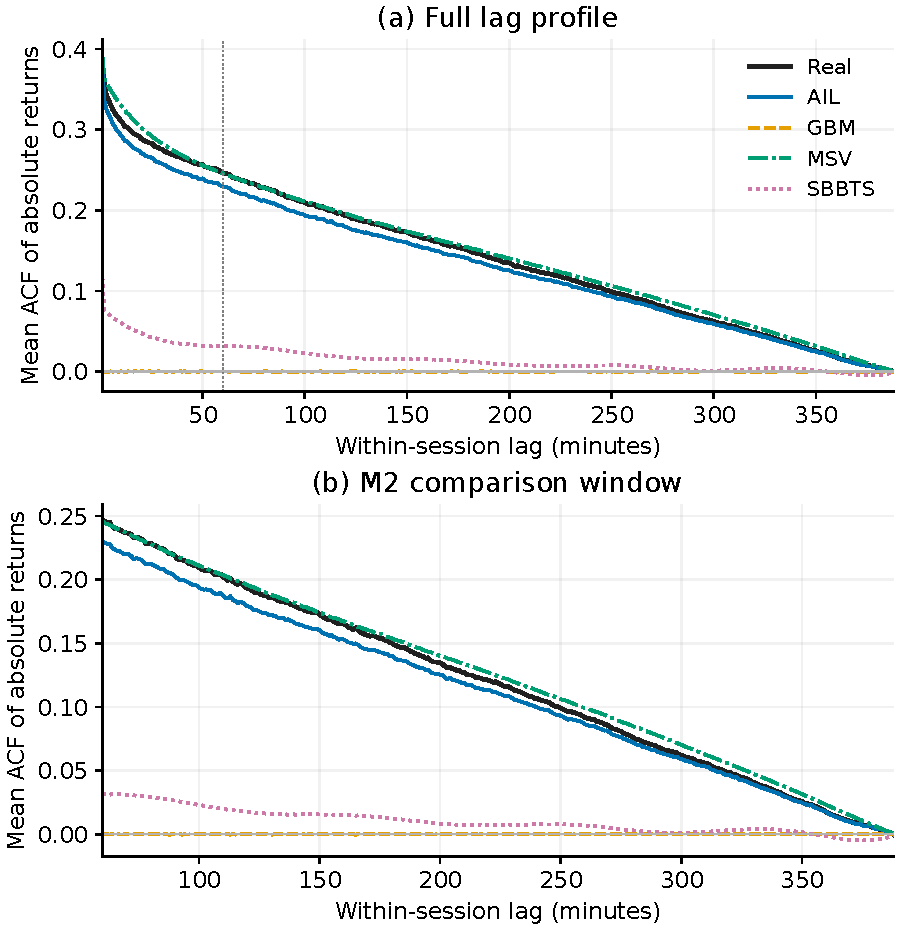
\includegraphics[width=\textwidth]{figures/m2_absolute_return_acf.pdf}
\caption{\edited{Absolute-return autocorrelation for the real and four
synthetic panels. Panel (a) shows lags 1--388 minutes; panel (b) isolates
the 60--388-minute window used by M2. Curves average ticker-level ACFs
over all 600 series, using within-session lagged products and full-sample
variance normalization. The resulting long-lag shrinkage is part of the
estimator. These are descriptive full-panel profiles, without uncertainty
bands, rather than matched-resampling scores. All panels cover the same
historical evaluation window, including SBBTS early-stopping dates.}}
\label{fig:m2-acf}
\end{figure}

MSV also scores above GBM on M1 ($0.0790$ versus $0.0184$).
Although both use Gaussian innovations, MSV's time-varying volatility
produces a scale mixture with heavier marginal tails.
Per-ticker standardization removes differences in unconditional scale
without removing this distributional distinction.
AIL has the highest point scores on M1, M3, and M4, but its profile
does not support uniform agreement with the empirical reference.
For the standardized marginal distribution, the score is $0.3436$
with interval $[0.2892,0.4292]$.
For volatility clustering, it is $0.2136$ with interval
$[0.1726,0.3482]$.
Both intervals lie below $0.5$, identifying discrepancies in marginal
return shape and persistent absolute-return dependence.
Because M2 uses an absolute distance between autocorrelation curves,
its score alone does not establish whether dependence is
under- or over-reproduced.
The same qualification now applies to aggregational Gaussianity:
AIL's M3 score is $0.3622$, with interval $[0.2445,0.4912]$.
This interval is comparatively wide and its upper endpoint lies close
to $0.5$, but the reported range remains below that reference.

Figure~\ref{fig:m3-kurtosis} separates the level of pooled kurtosis from
the normalized aggregation curve used by M3. AIL's normalized kurtosis
declines more rapidly than the real curve, whereas SBBTS becomes relatively
flat beyond five minutes. MSV exhibits a weaker decline and GBM remains
approximately flat. The raw and normalized panels are complementary:
closeness of normalized curves need not imply agreement in the level of
one-minute kurtosis.
\begin{figure}[tbp]
\centering
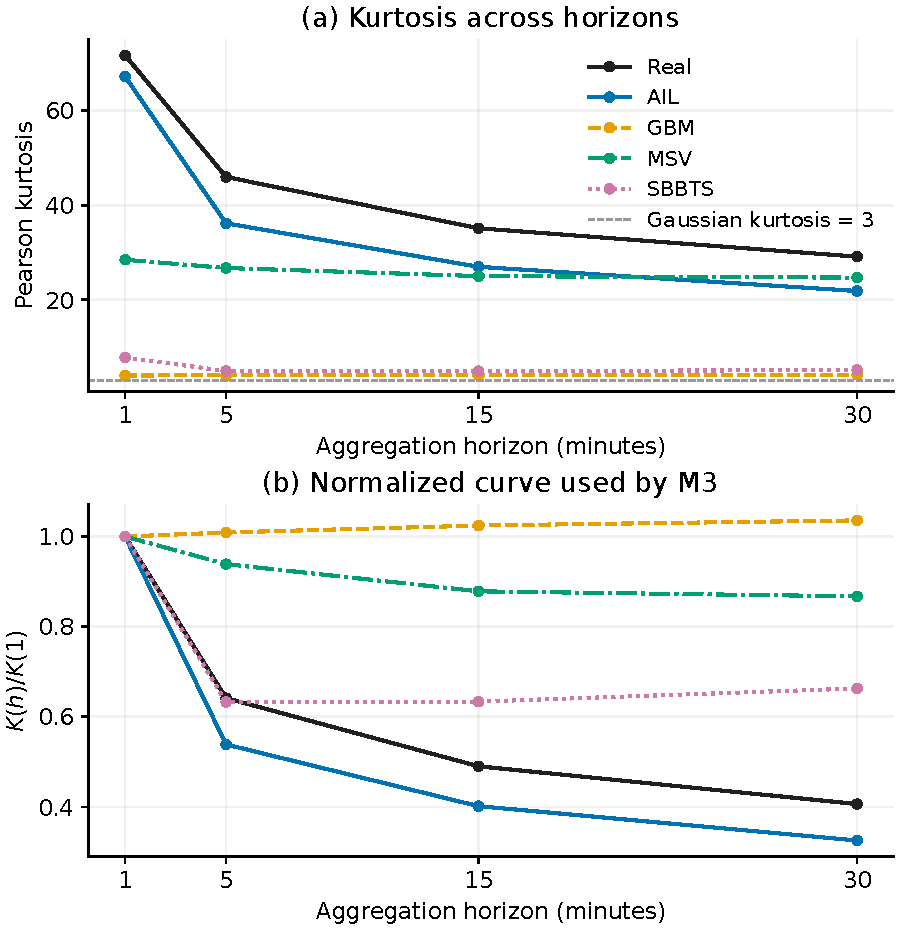
\includegraphics[width=\textwidth]{figures/m3_kurtosis_aggregation.pdf}
\caption{\edited{Kurtosis under temporal aggregation. Panel (a) reports
bias-corrected Pearson kurtosis of returns pooled across tickers and
sessions; the dashed reference is Gaussian kurtosis, 3. Panel (b) reports
$K(h)/K(1)$, the feature compared by M3, for horizons
$h\in\{1,5,15,30\}$ minutes. Every horizon uses the same final 360 return
positions of each eligible session. The two early-close sessions are
excluded, leaving 137 eligible sessions; blocks containing missing
observations are discarded. Lines connect evaluated horizons only.
The profiles use the full ticker panels and do not represent bootstrap
confidence intervals.}}
\label{fig:m3-kurtosis}
\end{figure}

For regime-conditional tails, AIL scores $0.4818$; its interval,
$[0.3922,0.5053]$, includes $0.5$.
M4 therefore does not clearly resolve a departure of the synthetic--real
gap from the real--real baseline at the reported interval level.
It does not establish equivalence: the interval also contains
scores materially below the reference.

\noindent\begin{minipage}{\textwidth}
The full-panel tail-shape profiles in Figure~\ref{fig:m4-xi} show close
alignment between AIL and the real panel across relative-volatility
quintiles. SBBTS yields smaller shape estimates throughout, while MSV's
profile rises markedly in its most turbulent quintile. These visual
comparisons concern tail shape conditional on each panel's own relative
volatility regime; they do not establish agreement in absolute volatility
thresholds, exceedance frequencies, or uncertainty about the fitted shapes.
\end{minipage}
\par
\begin{figure}[tbp]
\centering
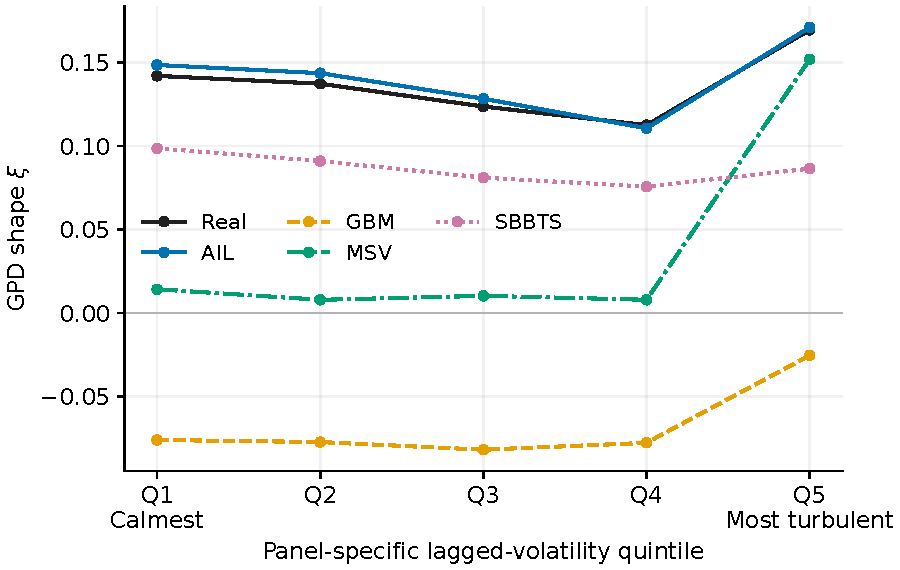
\includegraphics[width=\textwidth]{figures/m4_xi_by_regime.pdf}
\caption{\edited{Generalized Pareto shape $\xi$ across panel-specific
lagged-volatility quintiles, from Q1 (calmest) to Q5 (most turbulent).
Volatility uses a strictly lagged 60-minute within-session window with
at least 30 prior valid observations. Within each regime, the GPD is
fitted to excesses of absolute returns above their 95th percentile.
Quintiles and tail thresholds are fitted separately in each panel;
matching labels therefore denote relative ranks rather than equal
absolute volatility levels. The horizontal reference is $\xi=0$.
Lines join discrete full-panel estimates and imply no uncertainty bands.}}
\label{fig:m4-xi}
\end{figure}

SBBTS exhibits a different pattern.
Its M1 and M2 scores ($0.0245$ and $0.0203$) remain close to GBM,
indicating limited improvement over the Gaussian control on standardized
marginal shape and long-lag volatility dependence.
By contrast, its M3 and M4 scores ($0.2872$ and $0.1245$) exceed those
of both controls, placing it second to AIL on these properties.
All four SBBTS intervals nevertheless remain below $0.5$.
The gains on M3 and M4 thus represent relative improvements without
agreement with the empirical reference under the stated protocol.
The overlapping M3 intervals for AIL and SBBTS also warrant keeping
their point-score ordering distinct from a formal comparison of
their difference.
All original-panel point estimates, including GBM and SBBTS on M2,
lie within the reported intervals, although percentile intervals
are not required in general to contain the original estimate.
The aggregate deviation scores are $1.911$ for AIL, $6.561$ for MSV,
$13.532$ for SBBTS, and $28.031$ for GBM; lower values indicate
closer agreement with real--real gap parity.
Their respective intervals are $[1.522,2.325]$, $[5.541,7.277]$,
$[11.220,14.722]$, and $[23.750,30.219]$.
The aggregate ordering complements the individual metrics:
SBBTS improves on MSV for M3 and M4 while receiving a larger
aggregate deviation because of its discrepancies on M1 and M2.
The aggregate cannot identify that trade-off by itself.
The independent-seed analysis in Appendix~\ref{app:reproducibility}
separates numerical variation from corpus uncertainty.
Across all 20 seeds, AIL has the highest scores on M1, M3, and M4,
MSV has the highest M2 score, and the aggregate ordering remains
AIL, MSV, SBBTS, then GBM.
Absolute scores still vary with the inner resampling seed:
AIL's seed standard deviations are $0.0131$, $0.0141$, $0.0160$,
and $0.0166$ for M1--M4.
Its M4 seed range, $[0.4669,0.5277]$, crosses $0.5$.
These diagnostics support stability of the observed ordering under
inner resampling without establishing robustness to alternative
metric parameters, generator fits, or market periods.
}

% SENSITIVITY-VALIDATED: fixed 19-specification grid, five paired seeds.
\subsection{\edited{Sensitivity analysis}}\label{sec:sensitivity}
{\color{red}
Several metric parameters were selected during development with AIL outputs
visible. We therefore evaluate the frozen 19-specification grid on the same
four generators and fixed panels, using 100 matched draws and 200 tickers
per draw under each of five root seeds (42, 1, 2, 3, and 4).
The grid includes the primary specification, 15 single-parameter alternatives,
and three selected two-parameter combinations.
It varies M1 tail sharpness and magnitude, and M4's volatility window,
minimum-valid fraction, tail fraction, and regime weights.
The minimum-period rule is retained when the window or valid fraction changes.
Within each seed the specifications share the same sampled ticker indices.

The complete generator ordering is unchanged in all 45 paired comparisons
for M1 and all 45 for M4, and in all 90 aggregate comparisons.
Each metric comparison pairs one of nine affected alternatives with its
same-seed primary; the aggregate comparison covers all 18 alternatives.
No alternative moves a point score across the reference of 0.5 relative
to its same-seed primary.
Stable ordering does not imply unchanged scores.
For AIL, the paired score changes range from $-0.0452$ to $0.0144$ on M1
and from $-0.0378$ to $0.0181$ on M4.
Table~\ref{tab:sensitivity-ranges} reports the corresponding ranges for
all generators; Figures~\ref{fig:sensitivity-scores} and
\ref{fig:sensitivity-aggregate} show mean changes across seeds.
These are changes in point estimates; outer-bootstrap intervals are not
recomputed for the alternative specifications.

Only the affected metric is recomputed under each alternative; unchanged
same-seed metric results are reused and the aggregate is recalculated.
M2 and M3 parameters are held fixed, so their unchanged scores do not
demonstrate robustness to changes in those parameters.
The grid measures sensitivity within its specified ranges and selected
interactions. It does not establish robustness to every structural choice,
including the volatility-proxy family, or undo the AIL-informed selection
history. The primary specification is retained without selecting a new setting from
these outcomes.
}
